\chapter{Background}\label{chapter:background}

This section aims on providing a general overview of the various software tools that were used in this work. In particular, the FaaS platform that was deployed to the experimental edge computing cluster and the software components employed for monitoring purposes will be introduced.

\section{Docker}
\textit{Docker} is an Open-Source containerization platform developed by Docker Inc. which enables software developers to bundle an application together with any associated configuration files and other dependencies, which are required to be available at runtime in order to appropriately operate the software, into Docker images. In the context of containerization, images are standalone, executable software packages containing an isolated filesystem that act as an immutable blueprint for so-called containers, which are created once the respective image is executed. Containers are seperate, isolated processes that run on the host system and can be seen as the direct counterpart of Virtual Machines (VMs) due to the fact that they differ substantially in their characteristics and the way they function. For instance, containers are more lightweight and efficient because they utilize the kernel of the host's operating system (OS) instead of booting their own dedicated operating system, which results in a significant reduction of overhead and startup time. Furthermore, containers are highly portable because they only have to be created once in order to be deployed to any platform or environment as they are abstracted away from the OS of the host they run on. For example, Docker can be installed on Windows, Linux and macOS which makes it possible to deploy a containerized application to any of today's most common operating systems. Additionally, containerization completely eliminates the common problematic situation known from traditional software development where the software in question works in a certain environment, but falls into a faulty state when deployed to a different environment, due to the encapsulation of the application. Consequently, this accelerates productivity as it allows for a reproducible environment due to the fact that a container always behaves in the same way and is independent of the target platform and its surrounding. Lastly, Docker images can easily be shared with other developers by publishing it to an image registry such as Docker's \textit{DockerHub}, which is the world's largest repository service. 

The main component of Docker is the Docker Engine, which is a container runtime that acts as a client-server application and provides the following core features:

\begin{enumerate}
    \item \textit{Docker Daemon}: The Docker Daemon \textit{dockerd} is a persistent process that can be seen as the control plane of Docker. It is responsible for managing images, containers and other docker-related resources.
    \item \textit{Docker Engine API}: The Docker Engine offers a public RESTful API, which specifies interfaces that other programs can use in order to instruct the Docker daemon. These APIs can be accessed by any HTTP client.
    \item \textit{Command Line Interface (CLI)}: The Docker CLI named \textit{docker} acts as a client program that uses the provided APIs in order to communicate with the Docker daemon and can thus be used in order to build images, create or delete containers, pull an image from or push an image to a registry and more~\parencite{docker-engine}.
\end{enumerate}

Even though much of today's software is primarily designed to run on computers that are based on the x86-64 architecture, the situation of having to support different types of system architectures like ARM32v7 or its 64-bit based successor called ARM64v8 is not uncommon, especially in the case of IoT applications which are usually operated across a wide range of heterogeneous devices. To this end, Docker offers the possibility to execute multi-architecture builds for Docker images, which enables application developers to generate and publish multiple versions of a specific image at once, while each one is dedicated to a specific system architecture. Consequently, after uploading the produced images to an image registry, the containerized application can be deployed effortlessly to the intended devices.


\section{Kubernetes}
\textit{Kubernetes} is a famous Open-Source container orchestration tool first introduced by Google, which is designed to automate the deployment, load balancing, scaling and management of containerized applications. In Kubernetes, application containers run inside a so-called \textit{Pod} which is the smallest deployable unit provided by Kubernetes. Since it is a cluster-based software, it is typically used in a multi-node production environment in which each node performs the task of either the Master or Worker. While the former acts as the cluster's decision maker by hosting the master components of a cluster such as the \textit{kube-scheduler}, which is responsible for assigning a target node to newly created pods, or the key-value based backup store \textit{etcd} which incorporates all of the associated data of a cluster, the latter maintains the pods which are components of the application workload by communicating with the master nodes by the help of a running agent called \textit{kubelet} in order to take corresponding instructions. Hence, the application containers managed by Kubernetes are eventually deployed to a cluster's worker nodes~\parencite{k8s-components}.

The associated objects of a Kubernetes cluster are created and modified using configuration files which specify the currently desired state of one or more individual resources (e.g. a Pod). Even though both YAML and JSON are supported configuration languages, configuration files for Kubernetes are usually defined in YAML due to its better readability. Kubernetes provides a Command Line Interface named \usemintedstyle{bw}\mintinline{shell-session}|kubectl| which offers the possibility to apply such manifests to a specific cluster in order to create, adjust or delete the resources defined in the configuration file. Additionally, \usemintedstyle{bw}\mintinline{shell-session}|kubectl| serves as a cluster management tool that can be used for multiple purposes such as listing detailed information regarding the cluster and its resources or interacting with specific containers.

Kubernetes supports a wide range of container runtimes such as \textit{containerd} or any implementation of the \textit{Kubernetes Container Runtime} (CRI) like CRI-O~\parencite{k8s-components}. Even though Docker has recently been removed from the list of supported runtimes, applications that have been containerized using Docker can still be deployed to Kubernetes as long as they don't directly depend on features or settings that are explicitly provided by Docker~\parencite{k8s-docker-drop}.

In conclusion, the architecture of Kubernetes guarantees a great extensibility due to the fact that an existing cluster can easily be horizontally scaled by adding more worker nodes, which results in a highly-available, fault tolerant cluster. Similarly, this allows for an appropriate scaling of an application because an additional node supplies a Kubernetes cluster with necessary resources needed to deploy more replicas of the respective application to the cluster.

\section{Cluster Monitoring \& Data Visualization}
\subsection{Prometheus}
\textit{Prometheus} is an Open-Source, cutting-edge monitoring system that enables administrators to effectively supervise a system's infrastructure and associated applications. It is well known for its polling data collection model which regularly scrapes metrics over HTTP from the services being monitored, which are usually referred to as \textit{targets}, using a configurable time interval. Any data collected by a successful scrape is stored in a time-series database, which enables Prometheus to keep track of changes of the individual metrics over time. For the purpose of data selection and performing operations on the data, Prometheus provides an own query language called \textit{PromQL} which defines a wide range of functions that can be utilized in query expressions. Furthermore, it allows to define certain alert rules that are based on the collected data in order to trigger an alert once a specific condition defined in those rules is met. This allows for sending automatic notifications to administrating staff, which can then act appropriately based on what kind of alert has been triggered.

Generally, there is already a comprehensive amount of applications that natively expose metrics in the format expected by Prometheus. For any cases where this does not apply, a so-called data exporter can be employed, which is responsible for fetching data from third-party systems and transforming them into metrics that can be processed by Prometheus. Due to the fact that Prometheus offers a variety of client libraries which are available for a wide range of programming languages, custom exporters tailored to a specific use-case can easily be implemented.

\subsection{Grafana}
\textit{Grafana} is a modern Open-Source data analytics \& visualization platform that offers the possibility to plot data in a variety of ways using interactive, dynamic dashboards composed of a set of highly customizable widgets. To this end, the corresponding data can be obtained from a large selection of different data sources such as Prometheus, which is one of the most commonly used data sources for Grafana. Due to the fact that it provides the opportunity to construct an arbitrary amount of dashboards that are highly configurable, users are able to achieve a visualization of their data that satisfies individual requirements. Consequently, Grafana represents yet another powerful component of a modern system monitoring toolchain.

\section{OpenFaaS}
OpenFaaS is one of the most popular Open-Source FaaS platforms and is suitable for production-ready, large-scale applications due to the fact that it was designed to perfectly integrate with the commonly known industrial-strength container orchestration systems Kubernetes and OpenShift. Alternatively, in order to avoid the complexity of Kubernetes \textit{faasd} can be employed as an alternative, which is a lightweight version of OpenFaaS tailored to cost-sensitive or less complex and comprehensive projects~\parencite{openfaas-deployment}. OpenFaaS is very straightforward and easy to use as it supports a wide range of programming languages for serverless functions and only requires the user to package the serverless function into a container image that complies with the format defined by the \textit{Open Container Initiative} (OCI)~\parencite{openfaas-intro}. To this end, the OpenFaaS project provides a Command Line Interface named \textit{faas-cli}, which offers a variety of language templates that can be utilized to quickly build and deploy serverless functions. 

In OpenFaaS, serverless functions can be deployed and invoked by the \textit{API Gateway} which can be accessed via its REST API, the Web UI or the Command Line Interface. Additionally, serverless functions can also be invoked by more complex types of triggers like scheduled cron-jobs or third-party systems such as message brokers like \textit{Apache Kafka} or \textit{RabbitMQ}. For the latter, OpenFaaS offers so-called connectors that map a certain message topic to multiple functions, which offers the possibility to trigger an arbitrary amount of functions once a new message of the respective topic was received by the broker~\parencite{openfaas-triggers}. Figure \ref{fig:openfaas-gateway} provides an overview of the overall function invocation procedure and the individual components that are involved.

\begin{figure}[h]
    \centering
    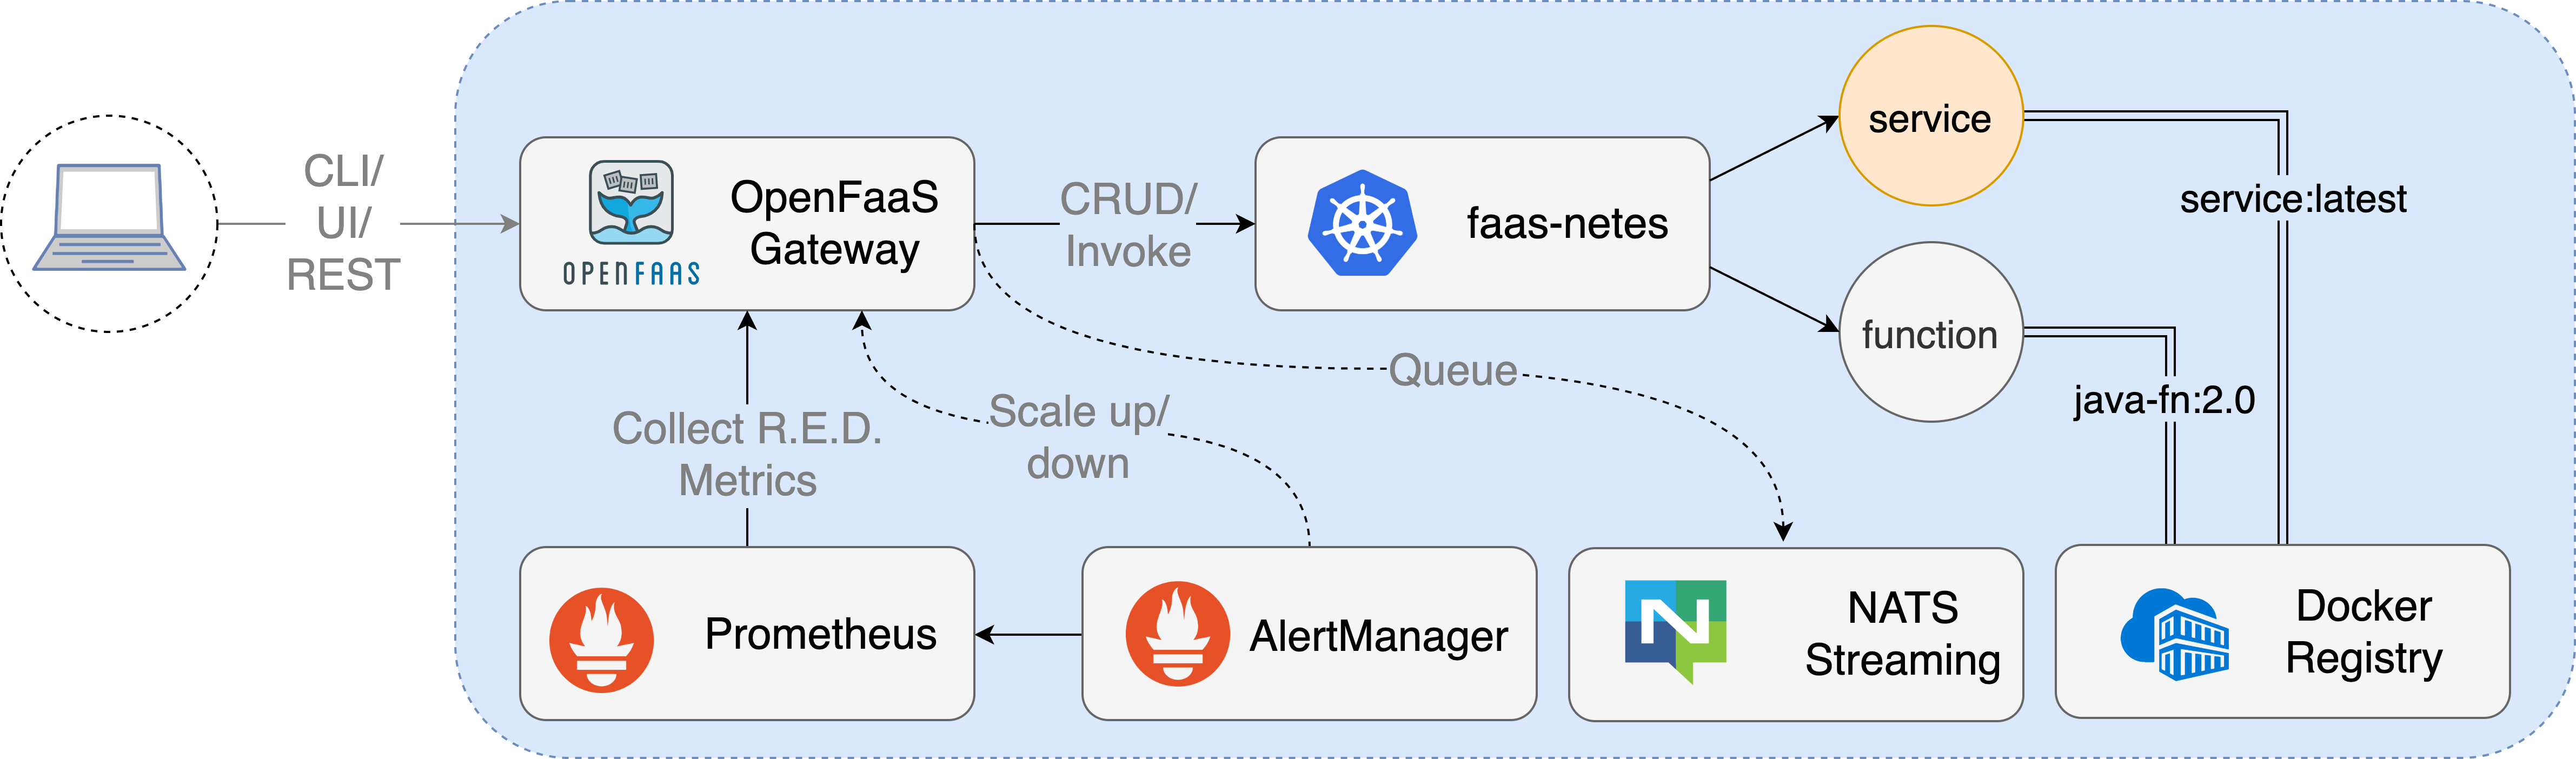
\includegraphics[width=1\textwidth]{./figures/of-workflow.png}
    \caption{Interaction with the OpenFaaS API Gateway~\parencite{openfaas-stack}}
    \label{fig:openfaas-gateway}
\end{figure}